%%%%%%%%%%%%%%%%%%%%%%%%%%%%%%%%%%%%%%%%%%%%%%%%%%%%%%%%%%%%%%%%%%%%%%%%%%%%%%%%%%
\begin{frame}[fragile]\frametitle{}
\begin{center}
{\Large Introduction to BharatVarsha (Geography)}
\end{center}
\end{frame}

%%%%%%%%%%%%%%%%%%%%%%%%%%%%%%%%%%%%%%%%%%%%%%%%%%%%%%%%%%%%%%%%%%%%%%%%%%%%%%%%%%
\begin{frame}[fragile]\frametitle{Geography of Ancient India}
\begin{columns}
\begin{column}{0.5\textwidth}
\begin{itemize}
   \item Diverse geographical features - Himalayas, Indo-Gangetic plain, peninsular plateau, and coastal regions.
   \item Strategic location at the intersection of Asia, Africa, and Europe.
   \item Abundance of natural resources - minerals, forests, and fertile agricultural lands.
   \item Network of major rivers - Indus, Ganges, Brahmaputra, and their tributaries.
   \item Varied climatic conditions - tropical, subtropical, and temperate.
\end{itemize}

\end{column}
\begin{column}{0.5\textwidth}
\begin{figure}
   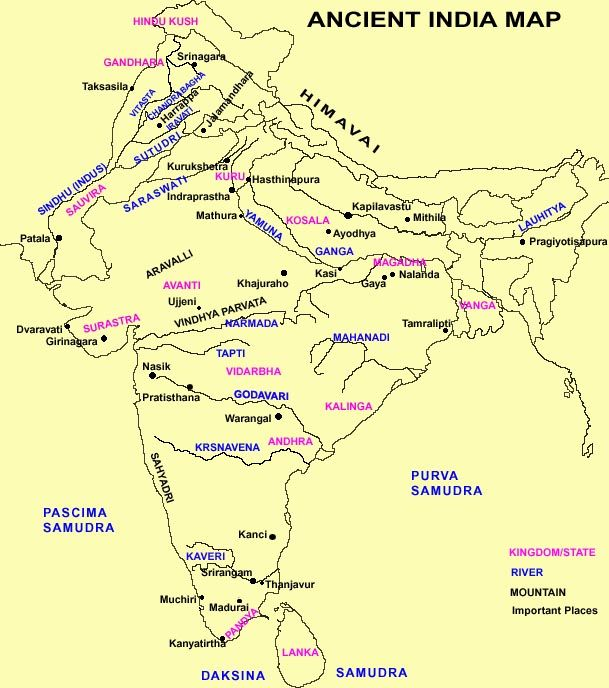
\includegraphics[width=\textwidth]{ancient_india_geography.jpg}
   \caption{Geography of Ancient India}
\end{figure}
\end{column}
\end{columns}
\end{frame}

%%%%%%%%%%%%%%%%%%%%%%%%%%%%%%%%%%%%%%%%%%%%%%%%%%%%%%%%%%%%%%%%%%%%%%%%%%%%%%%%%%
\begin{frame}[fragile]\frametitle{Geography of Ancient India}
\begin{columns}
\begin{column}{0.5\textwidth}
\begin{itemize}
   \item Rich biodiversity - home to a wide range of flora and fauna.
   \item Coastal regions with access to maritime trade routes.
   \item Diverse landscapes and ecosystems, including deserts, wetlands, and mountainous regions.
   \item Presence of important ancient cities and trade centers.
   \item Influence of geography on the development of ancient Indian civilizations and cultures.
\end{itemize}
\end{column}
\begin{column}{0.5\textwidth}
\begin{figure}
   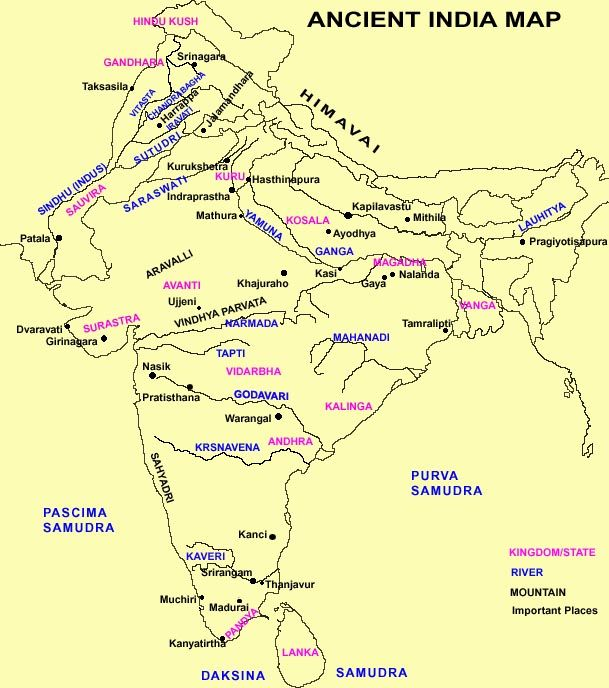
\includegraphics[width=\textwidth]{ancient_india_geography.jpg}
   \caption{Geography of Ancient India}
\end{figure}
\end{column}
\end{columns}
\end{frame}

%%%%%%%%%%%%%%%%%%%%%%%%%%%%%%%%%%%%%%%%%%%%%%%%%%%%%%%%%%%%%%%%%%%%%%%%%%%%%%%%%%
\begin{frame}[fragile]\frametitle{Geological Boundaries of India}
\begin{columns}
\begin{column}{0.5\textwidth}
\begin{itemize}
   \item Tectonic plates and geological formation of the Indian subcontinent.
   \item Himalayas: the northern mountain range formed by the collision of the Indian and Eurasian plates.
   \item Indo-Gangetic plain: the vast alluvial plain formed by the sediments carried by the major rivers.
   \item Peninsular India: the ancient, stable, and geologically diverse southern region.
   \item Deccan Plateau: the elevated plateau in the southern part of the Indian subcontinent.
   \item Coastal regions: the eastern and western coastlines shaped by the Arabian Sea and the Bay of Bengal.
\end{itemize}
\end{column}
\begin{column}{0.5\textwidth}
\begin{figure}
   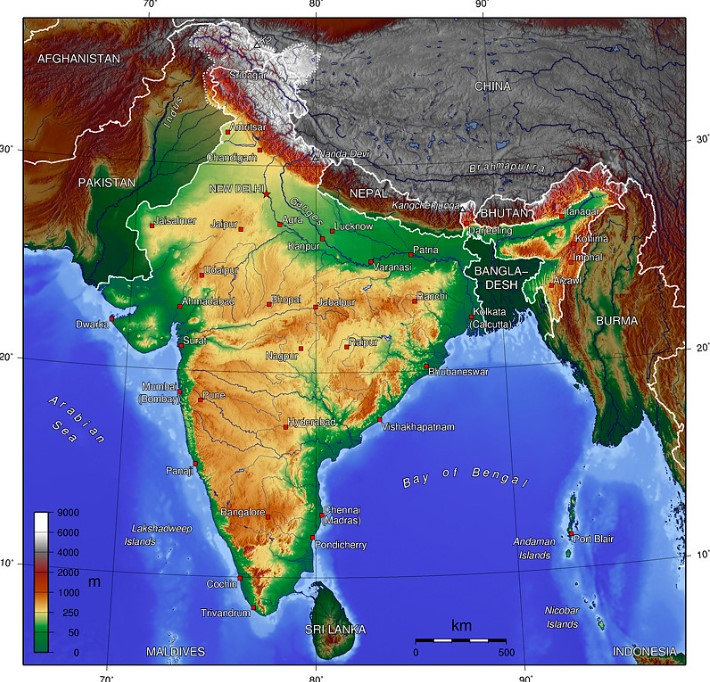
\includegraphics[width=\textwidth]{geological_boundaries_india.jpg}
   \caption{Geological Boundaries of India}
\end{figure}
\end{column}
\end{columns}
\end{frame}


%%%%%%%%%%%%%%%%%%%%%%%%%%%%%%%%%%%%%%%%%%%%%%%%%%%%%%%%%%%%%%%%%%%%%%%%%%%%%%%%%%
\begin{frame}[fragile]\frametitle{Geological Boundaries of India}
\begin{columns}
\begin{column}{0.5\textwidth}
\begin{itemize}
   \item Major geological faults and tectonic boundaries within the Indian landmass.
   \item Seismic activities and geological hazards associated with the Indian subcontinent.
   \item Mineral resources and their distribution across different geological regions.
   \item The influence of geological features on the cultural and economic development of ancient India.
\end{itemize}
\end{column}
\begin{column}{0.5\textwidth}
\begin{figure}
   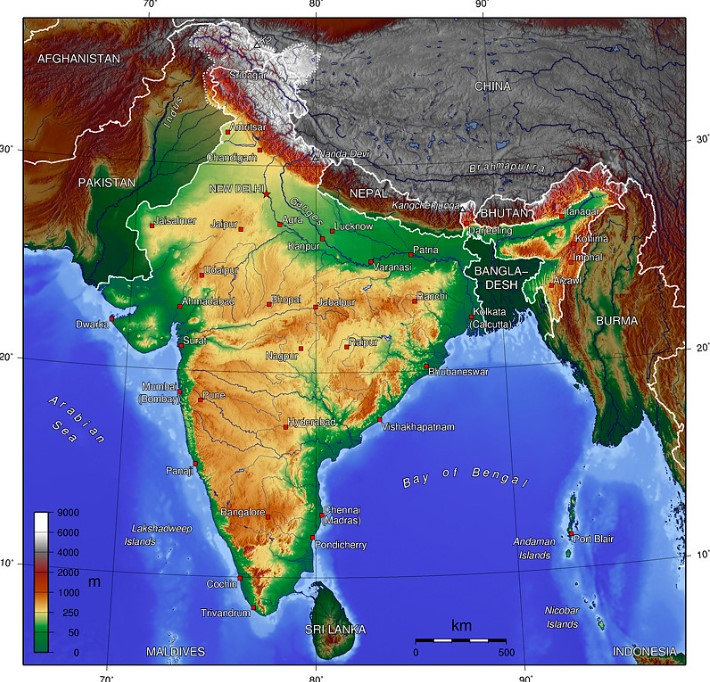
\includegraphics[width=\textwidth]{geological_boundaries_india.jpg}
   \caption{Geological Boundaries of India}
\end{figure}
\end{column}
\end{columns}
\end{frame}